\documentclass{article}
\usepackage[spanish]{babel}
\usepackage[utf8]{inputenc}
\usepackage[T1]{fontenc}
\usepackage{vmargin}
\usepackage{setspace}
\usepackage{enumerate}
\usepackage{graphicx}
\graphicspath{ {images/} }
\usepackage{float} 

\begin{document}
\begin{center}
\includegraphics[scale=0.3]{unison1.jpg}
\\
\vspace{0.5cm}
UNIVERSIDAD DE SONORA \\
\vspace{0.5cm}
DIVISIÓN DE CIENCIAS EXACTAS Y NATURALES \\
\vspace{0.5cm}
DEPARTAMENTO DE FÍSICA\\
\vspace{0.5cm}
LICENCIATURA EN FÍSICA\\
\vspace{0.5cm}
FÍSICA COMPUTACIONAL I

\vspace{2 cm}
\hrule
\vspace{1 cm}

{\huge \bfseries {Reporte de actividad 3}}
\\
\vspace{1 cm}
\hrule
\vspace{2 cm}
Ricardo Ruiz Hernández\\ 
\vspace{1 cm}
Profesor del curso\\
Dr. Carlos Lizárraga Celaya\\
\vspace{2 cm}
14 de febrero del 2018
\end{center}

\pagebreak
\begin{doublespace}

\hrule
\section{Introducción}
Esta práctica buscó involucrarnos más al mundo de Phyton y de Jupyter Notebook, de nueva cuenta, realizando gráficas en base a datos obtenidos de un sitio web, este último relacionado con aspectos del clima. A continuación se muestra el desarrollo de la práctica, anexando, al igual que la actividad pasada, los comandos utilizados, así como las gráficas resultantes.
\\
\hrule

\section{Contexto}
En el entendido de que en esta actividad se trabajará con un sondeo atmosférico, me parece pertinente definir este concepto.
\\
Un sondeo atmosférico es pues, un proceso en el que se obtienen datos sobre una determinada zona atmosférica; estos datos corresponden y describen propuedades físicas. El proceso es llevado a cabo por lo que se conoce como globo meteorológico. \\

Una de las utilidades que tiene conocer estas propiedades, es que se pueden realizar pronósticos del tiempo con mayor exactitud. 

\section{Análisis de datos}
Como primer paso visitamos el sitio de sondeos atmosféricos de la Universidad de Wyoming, seleccionamos una estación para después descargar los datos correspondientes a los días 22 de junio y 22 de diciembre, ambos del 2017. En mi caso, elegí Brindisi, Italia. \\
El archivo contenía columnas de valores de presión, altura, temperatura, temperatura de rocío, humedad reñativa, razón mixta, dirección de viento, velocidad del viento, además de otras variables termodinámicas.
\\
Abrimos una sesión en Jupyter, donde en la primera celda cargaremos las bibliotecas: \textit{Pandas, Numpy y Matplotlib.pyplot0}. 
Acto seguido leemos los datos, nombrando a su vez los dos txt: df1 para junio y df2 para diciembre, (df1 y df2 son comandos con los que se pueden mostrar los datos en una de las celdas).
\\
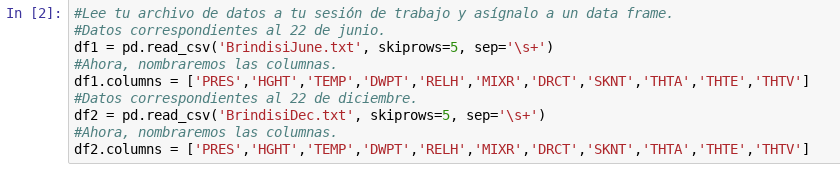
\includegraphics[scale=0.5]{act31.png}
\\
Una vez hecho esto, toca limpiar los datos, es decir, eliminar todos aquellos espacios vacíos que podrán entorpecer nuestos objetivos. En el caso de mis datos, no hubo problema.
Ahora bien, debemos verificar que nuestros datos sean valores numéricos; esto lo podemos hacer ejecutando el comando \textit{df1.dtypes} y \textit{df2.dtypes} para junio y diciembre, respectivamente.
\\
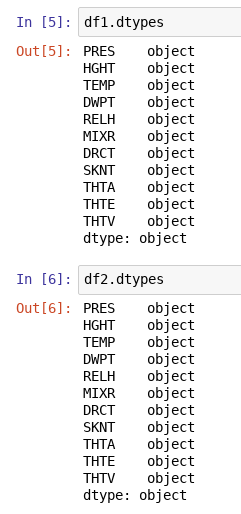
\includegraphics[scale=0.5]{act32.png}
\\
Como nos podemos percatar, se detectaron mis datos como objetos y no como valores numéricos, por lo que se recurrió a ejecutar un comando que transformara los objetos a números.
\\
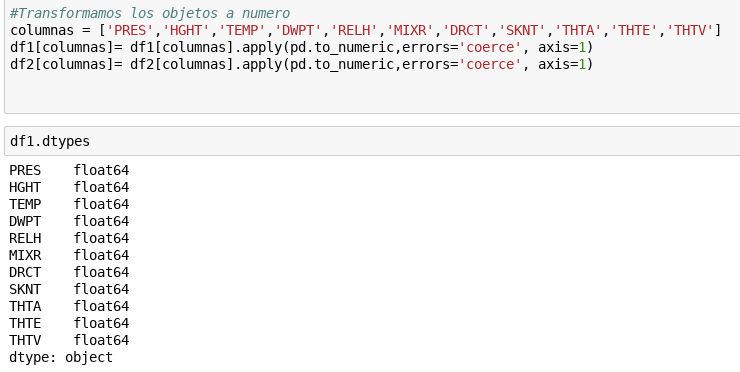
\includegraphics[scale=0.5]{act33.png}
\\
Con esto, podemos dar utilización a los datos, con la elaboración de gráficas.

\section{Resultados}
Se nos indica que se realice una gráfica de la presión con respecto a la altura, así como de la temperatura, igualmente, en función de la altura.
\\
A continuación muestro ambas gráficas:

	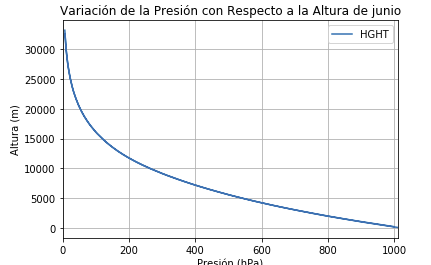
\includegraphics[height=5cm]{act35.png}  \hspace*{\fill}
    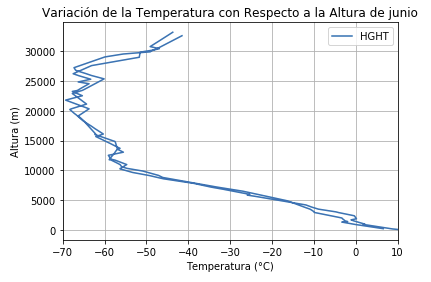
\includegraphics[height=5cm]{act37.png}
\\
\begin{itemize}


\item Y sus respectivos códigos: 
\\
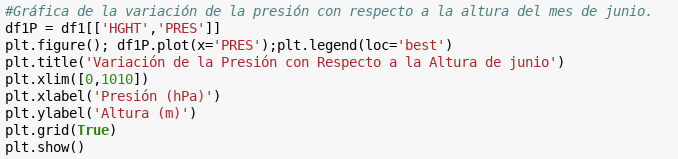
\includegraphics[height=1.7cm]{act34.png}  \hspace*{\fill}
    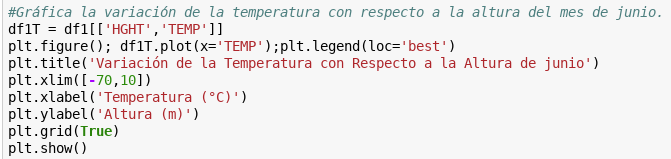
\includegraphics[height=1.7cm]{act36.png}
    
\item Estas gráficas son correspondientes al mes de junio, ahora mostraré los resultados de diciembre:
\\
	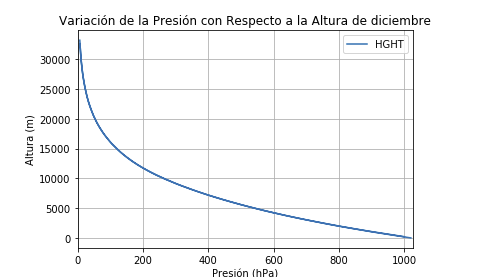
\includegraphics[height=5cm]{act39.png}  \hspace*{\fill}
    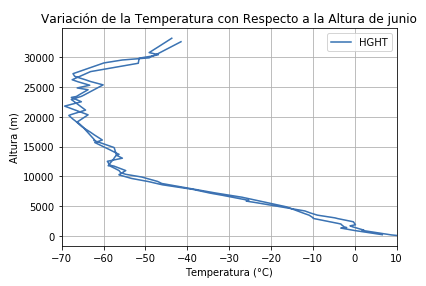
\includegraphics[height=5cm]{act311.png}

\item Y sus respectivos códigos:
\\
	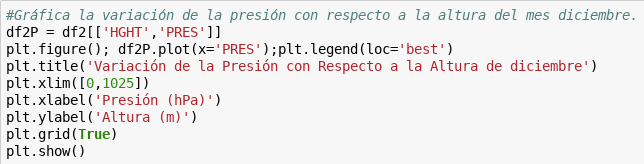
\includegraphics[height=1.7cm]{act38.png}  \hspace*{\fill}
    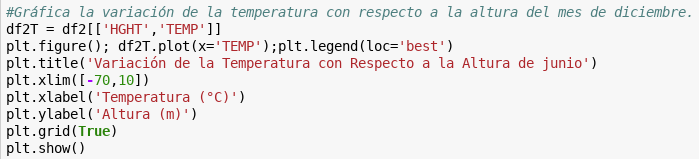
\includegraphics[height=1.7cm]{act310.png}
      \\
Se nos cuestiona lo siguiente, en relación con las gráficas de variación de la temperatura con respecto a la altura: \textit{¿Hay cambios significativos en la tropopausa entre las dos fechas?}
\\
Curiosamente la respuesta es no. Analizando la zona que corresponde a la tropopausa (entre los 9 y 17 km de altura) vemos un comportamiento en ambas gráficas muy parecido.


\item De manera análoga, se nos pide hacer gráficas más para cada mes, siendo la primera de ellas una gráfica de la temperatura (TEMP) y temperatura de rocío (DEWPT), como función de la altura; misma que resultó de la siguiente manera:
\\
	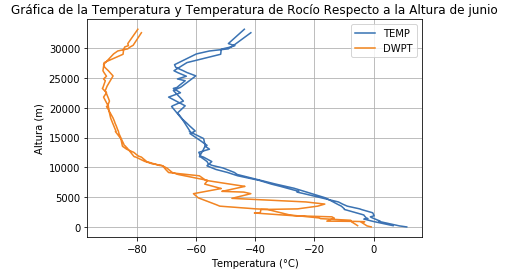
\includegraphics[height=4cm]{act312.png}  \hspace*{\fill}
    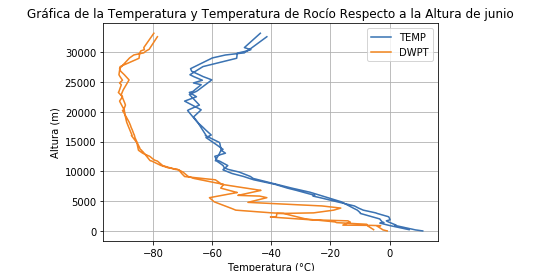
\includegraphics[height=4cm]{act313.png}
\item Lo siguiente fue realizar una gráfica de la rapidez de los vientos en nudos (SKNT).
\\
	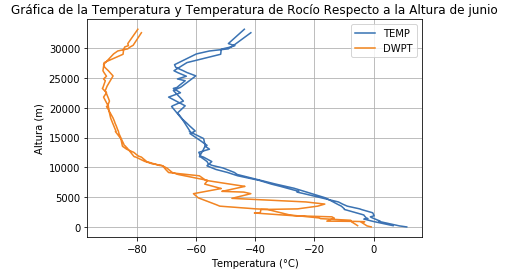
\includegraphics[height=4cm]{act312.png}  \hspace*{\fill}
    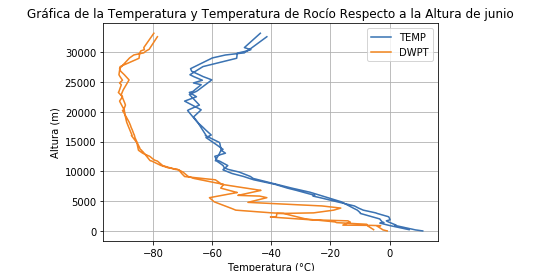
\includegraphics[height=4cm]{act313.png}
\item Por último tenemos las gráficas de la humedad relativa en función de la altura.
\\
	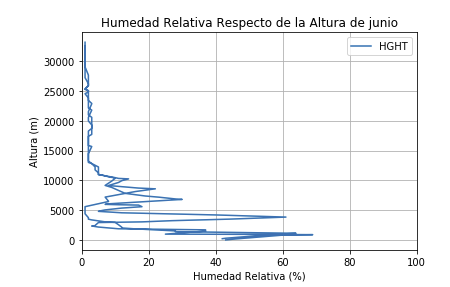
\includegraphics[height=4cm]{act316.png}  \hspace*{\fill}
    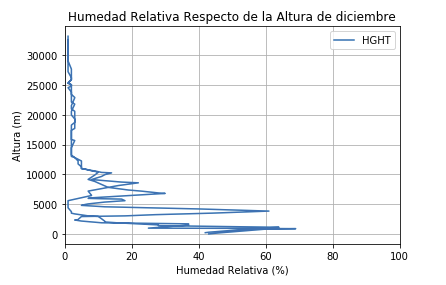
\includegraphics[height=4cm]{act317.png}

\section{Conclusión}
Esta sesión distó de ser sencilla, puesto que involucra nuevos conceptos con respecto a la anterior, tales como la limpieza de datos, nombramiento y organización de los mismos. Todo esto para evitar errores en nuestras gráficas. Este último proceso me resultó más sencillo esta vez, puesto que se trataba de mi segunda experiencia, y aunque hubo aspectos nuevos, se resolvieron sin problemas mayúsculos.
\\
Pienso que se cumple el objetivo de la práctica, de aprender  a dar estructura a los datos.

\section{Bibliografía}

\section{Apéndice}
\begin{enumerate}
\item \textit{¿Cuál es tu opinión general de esta actividad?}
\\
Me resultó buena, pues complementa los conocimientos de la actividad anterior.

\item \textit{¿Qué fue lo que más te agradó? ¿Lo que menos te agradó?}
\\
Me agrada el hecho de poder manejar una gran cantidad de datos sin dificultad alguna; si debo apuntar algo negativo sería que resulta tedioso en principio el proceso de estructuración y limpieza, pero al percatarte de que es necesario, te adaptas.

\item \textit{¿Que consideras que aprendiste en esta actividad?}
\\
Lo más relevante fueron los comandos para analizar y depurar datos.

\item \textit{¿Qué le faltó? ¿O le sobró?}
\\
No le quitaría ni agregaría nada.

\item \textit{¿Que mejoras sugieres a la actividad?}
\\
Una base donde recargarnos, puesto que, lleva mucho tiempo encontrar el comando y la forma correcta, podría decir que algun sitio web donde obtener información al respecto.
\end{enumerate}


\end{itemize}
\end{doublespace}
\end{document}
